\section{Cronograma}

Inicialmente realizamos un cronograma tentativo de la totalidad del trabajo, incluyendo el desarrollo de cada caso de uso, el despliegue en cada ecosistema y su documentación asociada como se muestra en la Figura \ref{fig:cronograma-tentativo}. Sin embargo, a medida que fuimos desarrollando el trabajo nos encontramos con que dividir el trabajo por ecosistemas era más eficiente que dividirlo por casos de usos como en nuestro cronograma estimado.

\begin{figure}[H]
    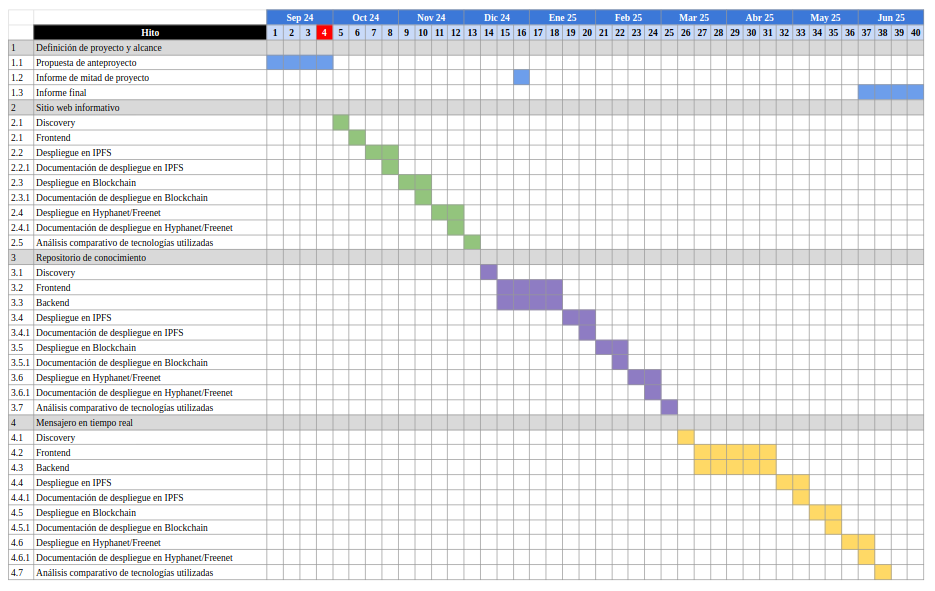
\includegraphics[width=1\linewidth]{img/cronograma.png}
    \caption{Cronograma tentativo}
    \label{fig:cronograma-tentativo}
\end{figure}

Por lo tanto, lo que terminó sucediendo es lo que se muestra en la Figura \ref{fig:cronograma-real}. La división se hizo por ecosistema, esto incluye la investigación, el desarrollo y la documentación de cada caso de uso para el ecosistema en cuestión. Hacerlo de esta manera nos permitió paralelizar los esfuerzos y evitamos superposiciones durante la investigación y desarrollo. Esta separación podría haber generado silos de conocimiento por ecosistema dentro del equipo, es por esto que las reuniones semanales de puesta en común, junto con la constante comunicación por chat y sesiones de \textit{pair-programming}, fueron de vital importancia para mitigar dicha separación y que todo el equipo esté al tanto de los conocimientos adquiridos de cada ecosistema.

\begin{figure}[H]
    \centering
    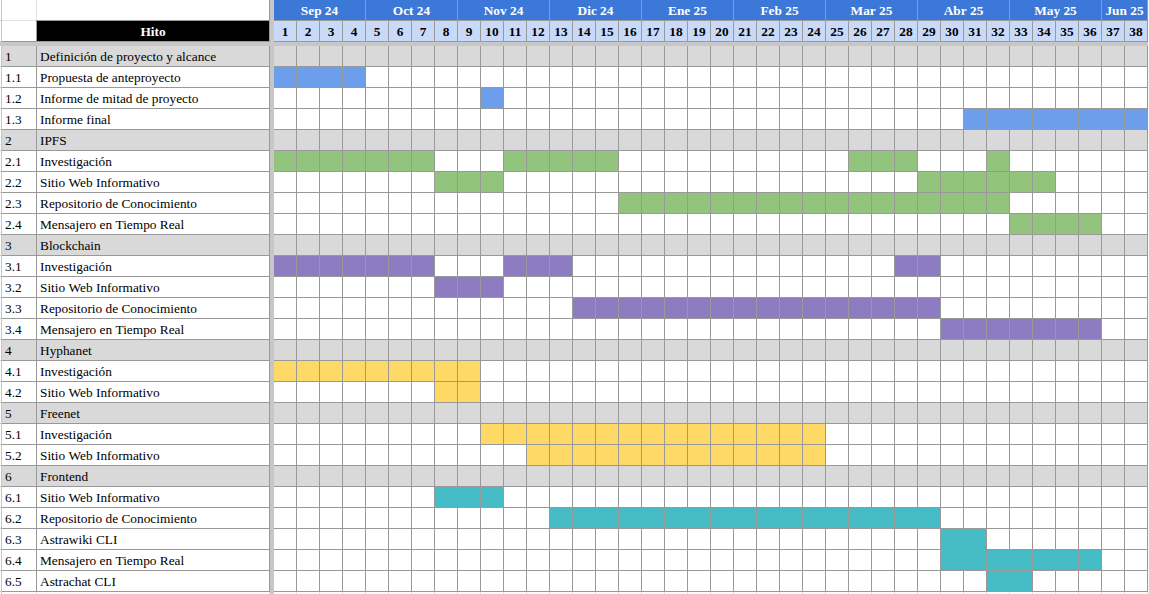
\includegraphics[width=1\linewidth]{img/cronograma-real.png}
    \caption{Cronograma real}
    \label{fig:cronograma-real}
\end{figure}


% \begin{enumerate}

%     \item \textbf{Definición de proyecto y alcance}
%     \begin{enumerate}[label*=\arabic*.]
%         \item Propuesta de anteproyecto (Semanas 1 a 4)
%         \item Informe de mitad de proyecto (Semanas 16 a 17)
%         \item Informe final (Semanas 37 a 40)
%     \end{enumerate}
    
%     \item \textbf{Sitio web informativo} (Semanas 5 a 13)
%     \begin{enumerate}[label*=\arabic*.]
%         \item Discovery
%         \item Frontend
%         \item Despliegue en IPFS
%         \begin{enumerate}[label*=\arabic*.]
%             \item Documentación de despliegue en IPFS
%         \end{enumerate}
%         \item Despliegue en Blockchain
%         \begin{enumerate}[label*=\arabic*.]
%             \item Documentación de despliegue en Blockchain
%         \end{enumerate}
%         \item Despliegue en Hyphanet/Freenet
%         \begin{enumerate}[label*=\arabic*.]
%             \item Documentación de despliegue en Hyphanet/Freenet
%         \end{enumerate}
%         \item Análisis comparativo de tecnologías utilizadas
%     \end{enumerate}
    
%     \item \textbf{Repositorio de conocimiento} (Semanas 14 a 25)
%     \begin{enumerate}[label*=\arabic*.]
%         \item Discovery
%         \item Frontend
%         \item Backend
%         \item Despliegue en IPFS
%         \begin{enumerate}[label*=\arabic*.]
%             \item Documentación de despliegue en IPFS
%         \end{enumerate}
%         \item Despliegue en Blockchain
%         \begin{enumerate}[label*=\arabic*.]
%             \item Documentación de despliegue en Blockchain
%         \end{enumerate}
%         \item Despliegue en Hyphanet/Freenet
%         \begin{enumerate}[label*=\arabic*.]
%             \item Documentación de despliegue en Hyphanet/Freenet
%         \end{enumerate}
%         \item Análisis comparativo de tecnologías utilizadas
%     \end{enumerate}
    
%     \item \textbf{Mensajero en tiempo real} (Semanas 26 a 38)
%     \begin{enumerate}[label*=\arabic*.]
%         \item Discovery
%         \item Frontend
%         \item Backend
%         \item Despliegue en IPFS
%         \begin{enumerate}[label*=\arabic*.]
%             \item Documentación de despliegue en IPFS
%         \end{enumerate}
%         \item Despliegue en Blockchain
%         \begin{enumerate}[label*=\arabic*.]
%             \item Documentación de despliegue en Blockchain
%         \end{enumerate}
%         \item Despliegue en Hyphanet/Freenet
%         \begin{enumerate}[label*=\arabic*.]
%             \item Documentación de despliegue en Hyphanet/Freenet
%         \end{enumerate}
%         \item Análisis comparativo de tecnologías utilizadas
%     \end{enumerate}

% \end{enumerate}